%\documentclass{report}
% Change "article" to "report" to get rid of page number on title page
\documentclass[fleqn]{article}

\usepackage{graphicx}
\usepackage{graphicx}

\usepackage{amsmath,amsfonts,amsthm,amssymb,dsfont}
\usepackage{setspace}
\usepackage{Tabbing}
\usepackage{fancyhdr}
\usepackage{lastpage}
\usepackage{extramarks}
\usepackage{chngpage}
\usepackage{soul,color}
\usepackage{graphicx,float,wrapfig}
\usepackage{enumitem}
\usepackage{url}
\usepackage{lipsum}
\usepackage{hanging}
\usepackage{mdframed}               %%%%   for breakable box answers
\usepackage[most]{tcolorbox}        %%%%   for breakable enhanced box answers
\usepackage{amsmath}
%\usepackage{pdfcomment}
%\usepackage[pdftitle={Homework 1},pdflang=en-US]{hyperref}
%%%\usepackage{axessibility}
%%%\usepackage{accsupp}
%%%\usepackage{amssymb}
%%%\usepackage{xstring}


% In case you need to adjust margins:
\topmargin=-0.45in      %
\evensidemargin=0in     %
\oddsidemargin=0in      %
\textwidth=6.5in        %
\textheight=9.0in       %
\headsep=0.25in         %

% Homework Specific Information
\newcommand{\hmwkTitle}{Homework 1}
\newcommand{\hmwkDueDate}{February 20 @ 4:00pm}
\newcommand{\hmwkClass}{CS 485/685}
\newcommand{\hmwkClassName}{Computer Vision}
\newcommand{\hmwkClassCode}{CS 485/685}
\newcommand{\hmwkAuthorName}{}

% Setup the header and footer
\pagestyle{fancy}                                                       %
\lhead{\sf\textbf\hmwkClass}                                            %
\chead{\Large\sf\textbf\hmwkTitle}                                      %
\rhead{Due: \sf\textbf\hmwkDueDate}                                     %
\lfoot{\lastxmark}                                                      %
\cfoot{}                                                                %
\rfoot{Page\ \thepage\ of\ \pageref{LastPage}}                          %
\renewcommand\headrulewidth{0.4pt}                                      %
\renewcommand\footrulewidth{0.4pt}                                      %

% This is used to trace down (pin point) problems
% in latexing a document:
%\tracingall

%%%%%%%%%%%%%%%%%%%%%%%%%%%%%%%%%%%%%%%%%%%%%%%%%%%%%%%%%%%%%
% Some tools
\newcommand{\enterProblemHeader}[1]{\nobreak\extramarks{#1}{#1 continued on next page\ldots}\nobreak%
                                    \nobreak\extramarks{#1 (continued)}{#1 continued on next page\ldots}\nobreak}%
\newcommand{\exitProblemHeader}[1]{\nobreak\extramarks{#1 (continued)}{#1 continued on next page\ldots}\nobreak%
                                   \nobreak\extramarks{#1}{}\nobreak}%

\newlength{\labelLength}
\newcommand{\labelAnswer}[2]
  {\settowidth{\labelLength}{#1}%
   \addtolength{\labelLength}{0.25in}%
   \changetext{}{-\labelLength}{}{}{}%
   \noindent\fbox{\begin{minipage}[c]{\columnwidth}#2\end{minipage}}%
   \marginpar{\fbox{#1}}%

   % We put the blank space above in order to make sure this
   % \marginpar gets correctly placed.
   \changetext{}{+\labelLength}{}{}{}}%

\setcounter{secnumdepth}{0}
\newcommand{\homeworkProblemName}{}%
\newcounter{homeworkProblemCounter}%
\newenvironment{homeworkProblem}[1][Problem \arabic{homeworkProblemCounter}]%
  {\stepcounter{homeworkProblemCounter}%
   \renewcommand{\homeworkProblemName}{#1}%
   \section{\homeworkProblemName}%
   \enterProblemHeader{\homeworkProblemName}}%
  {\exitProblemHeader{\homeworkProblemName}}%

\newcommand{\problemAnswer}[1]
  {\noindent\begin{mdframed}{#1}\end{mdframed}}%
%  {\noindent\fbox{\begin{minipage}[c]{\columnwidth}#1\end{minipage}}}%

\newcommand{\problemAnswerEnhanced}[1]
  {\noindent\begin{tcolorbox}[breakable, enhanced] {Answer:\\#1}\end{tcolorbox}}%
%  {\noindent\fbox{\begin{minipage}[c]{\columnwidth}#1\end{minipage}}}%


\newcommand{\problemLAnswer}[1]
  {\labelAnswer{\homeworkProblemName}{#1}}

\newcommand{\homeworkSectionName}{}%
\newlength{\homeworkSectionLabelLength}{}%
\newenvironment{homeworkSection}[1]%
  {% We put this space here to make sure we're not connected to the above.
   % Otherwise the changetext can do funny things to the other margin

   \renewcommand{\homeworkSectionName}{#1}%
   \settowidth{\homeworkSectionLabelLength}{\homeworkSectionName}%
   \addtolength{\homeworkSectionLabelLength}{0.25in}%
   \changetext{}{-\homeworkSectionLabelLength}{}{}{}%
   \subsection{\homeworkSectionName}%
   \enterProblemHeader{\homeworkProblemName\ [\homeworkSectionName]}}%
  {\enterProblemHeader{\homeworkProblemName}%

   % We put the blank space above in order to make sure this margin
   % change doesn't happen too soon (otherwise \sectionAnswer's can
   % get ugly about their \marginpar placement.
   \changetext{}{+\homeworkSectionLabelLength}{}{}{}}%

\newcommand{\sectionAnswer}[1]
  {% We put this space here to make sure we're disconnected from the previous
   % passage

   \noindent\fbox{\begin{minipage}[c]{\columnwidth}#1\end{minipage}}%
   \enterProblemHeader{\homeworkProblemName}\exitProblemHeader{\homeworkProblemName}%
   \marginpar{\fbox{\homeworkSectionName}}%

   % We put the blank space above in order to make sure this
   % \marginpar gets correctly placed.
   }%

%%%%%%%%%%%%%%%%%%%%%%%%%%%%%%%%%%%%%%%%%%%%%%%%%%%%%%%%%%%%%


%%%%%%%%%%%%%%%%%%%%%%%%%%%%%%%%%%%%%%%%%%%%%%%%%%%%%%%%%%%%%
% Make title
\title{\vspace{1in}
\hrule
\vspace{.5in}
{\Huge{\textbf{\hmwkTitle}}}\\
\LARGE\vspace{0.1in}{Due\ on\ \hmwkDueDate}\\
\vspace{0.1in}\Large{\textit{\hmwkClass\ -- \hmwkClassName}}\vspace{0.5in}\hrule\vspace{2in}}
\date{}
\author{\textbf{\hmwkAuthorName}}
%%%%%%%%%%%%%%%%%%%%%%%%%%%%%%%%%%%%%%%%%%%%%%%%%%%%%%%%%%%%%

\begin{document}
\begin{spacing}{1.1}
\maketitle
\newpage
% Uncomment the \tableofcontents and \newpage lines to get a Contents page
% Uncomment the \setcounter line as well if you do NOT want subsections
%       listed in Contents
%\setcounter{tocdepth}{1}
%\tableofcontents
%\newpage

% When problems are long, it may be desirable to put a \newpage or a
% \clearpage before each homeworkProblem environment

\clearpage
\begin{homeworkProblem}
{\sf\textbf{[20 pts]} }\textbf{Self Assessment Questions:}  In this problem, you will review the lecture from unit 02- Math Review. After studying the topics covered, you will design the following questions. For each of your questions, you will provide the correct answers with the rationale behind each answer.

\begin{enumerate}[label=\bfseries \alph*)]
    \item {\sf\textbf{[4 pts]} }Design and answer four (4) multiple choice questions. 
    \item {\sf\textbf{[6 pts]} }Design and answer two (2) fill in the blank questions.
    \item {\sf\textbf{[10 pts]} }Design and answer two (2) mathematical proof questions, mathematical computation questions, or a both.
\end{enumerate}


%%%%% Your Answer here:
\problemAnswerEnhanced{
\begin{enumerate}[label=\bfseries \alph*)]
    \item Design and answer four (4) multiple choice questions:
        \begin{itemize}
            \item 1. What are two main uses of Vectors?
            	\subitem a) Picture, Pixel
            	\subitem b) gradient, offsets
            	\subitem c) Data, Geometric representation 
            	\subitem d) gradient, Geometric representation  $\leftarrow$ \textbf{Answer}
            	
            \item 2. Dot product of two vectors is a 
                \subitem a) vector
            	\subitem b) integer
            	\subitem c) point 
            	\subitem d) scalar  $\leftarrow$ \textbf{Answer}
            
            \item 3. Vectors can be expressed as what combinations of the unit vectors?
                \subitem a) linear  $\leftarrow$ \textbf{Answer}
            	\subitem b) non-linear
            	\subitem c)  Geometric  
            	\subitem d) Gradient
            
            \item 4. When can we say a set of vectors are linearly dependent
                \subitem a) at least one is a non linear combination of the other
            	\subitem b) at least one is a linear combination of the other $\leftarrow$ \textbf{Answer}
            	\subitem c) more than one is a Geometric representation of the other
            	\subitem d) none of the above
            
        \end{itemize}
    \item Design and answer two (2) fill in the blank questions:
        \begin{itemize}
            \item 2D and 3D offsets can be represented by \quad \quad \quad .
            	\subitem \textbf{vectors}
            \item Points are \quad \quad \quad from the origin
            	\subitem \textbf{vectors}
        \end{itemize}
    \item Design and answer two (2) mathematical proof questions, mathematical computation questions, or a both:
        \begin{itemize}
            \item prove $ \vec{u}\cdot (\vec{v}+ \vec{w} ) =  \vec{u} \cdot \vec{v} + \vec{u} + \vec{w} $
            \begin{flalign*}\vec u\centerdot \left( {\vec v + \vec w} \right) & = \left\langle {{u_1},{u_2}, \ldots ,{u_n}} \right\rangle \centerdot \left( {\left\langle {{v_1},{v_2}, \ldots ,{v_n}} \right\rangle  + \left\langle {{w_1},{w_2}, \ldots ,{w_n}} \right\rangle } \right)\\ &  = \left\langle {{u_1},{u_2}, \ldots ,{u_n}} \right\rangle \centerdot \left\langle {{v_1} + {w_1},{v_2} + {w_2}, \ldots ,{v_n} + {w_n}} \right\rangle \\ &  =  {{u_1}\left( {{v_1} + {w_1}} \right),{u_2}\left( {{v_2} + {w_2}} \right), \ldots ,{u_n}\left( {{v_n} + {w_n}} \right)}  \\ &  =  {{u_1}{v_1} + {u_1}{w_1},{u_2}{v_2} + {u_2}{w_2}, \ldots ,{u_n}{v_n} + {u_n}{w_n}}  \\ &  = \left( {{u_1}{v_1},{u_2}{v_2}, \ldots 
            	,{u_n}{v_n}} \right)  + \left( {{u_1}{w_1},{u_2}{w_2}, \ldots ,{u_n}{w_n}} \right) \\ &  = \left\langle {{u_1},{u_2}, \ldots ,{u_n}} \right\rangle \centerdot \left\langle {{v_1},{v_2}, \ldots ,{v_n}} \right\rangle  + \left\langle {{u_1},{u_2}, \ldots ,{u_n}} \right\rangle \centerdot \left\langle {{w_1},{w_2}, \ldots ,{w_n}} \right\rangle \\ &  = \vec u\centerdot \vec v + \vec u\centerdot \vec w
            \end{flalign*}
            \item prove $\vec{v} \cdot \vec{v} = 0 \rightarrowtail \vec{v} = 0$
            \begin{flalign*}\vec v\centerdot \vec v & = \left\langle {{v_1},{v_2}, \ldots ,{v_n}} \right\rangle \centerdot \left\langle {{v_1},{v_2}, \ldots ,{v_n}} \right\rangle \\ &  = v_1^2 + v_2^2 +  \cdots  + v_n^2\\ &  = 0
            \end{flalign*}
        \end{itemize}
\end{enumerate}
}

\end{homeworkProblem}


\pagebreak


\begin{homeworkProblem}
 {\sf\textbf{[20 pts]} } 
 
 \begin{equation}
 \mathbf{A}^T=\left[1\quad2\quad3\right],\qquad \mathbf{B}^T=\left[2 \quad 1 \quad3\right] \qquad \textrm{and}\qquad \mathbf{C}^T=\left[1 \quad 3 \quad2\right]
 \end{equation}
 
 
 Answer the following questions:
 
\begin{enumerate}[label=\bfseries \alph*)]
    \item  {\sf\textbf{[5 pts]} }Do the vectors $A, B$, and $C$ span $\mathbb R^3$? Why?
    \item  {\sf\textbf{[10 pts]} }If the vectors above span $\mathbb R^3$, find the orthonormal basis vectors corresponding to each. If they don't span $\mathbb R^3$, modify one of the vectors and then find the orthonormal basis vectors corresponding to each. 
    \item {\sf\textbf{[5 pts]} }Find the expansion of the vector $V^T=\left[6\quad8\quad-4\right]$ in the orthonormal basis vector above.
\end{enumerate}


%%%%% Your Answer here:
\problemAnswerEnhanced{
\begin{enumerate}[label=\bfseries \alph*)]
    \item Calculating matrix rank 
   \[
   \begin{bmatrix}
   1    &2 & 3  \\
   2    &1 & 3  \\
   1    & 3 &2 
      \end{bmatrix}
   =
   \begin{bmatrix}
1    &2 & 3  \\
0    &-3 & -3  \\
0    & 0 &-2 
\end{bmatrix}
\rightarrow \text{Rank } \rightarrow 3
   \]
   Yes they span over $R^3$  it is clear the rank of the matrix is 3, so the vectors span a subspace of dimension 3
    \item 
    \[
    \mathbf{u_k}=\mathbf{v_k}-\sum_{j=1}^{k-1}\text{proj}_{\mathbf{u_j}}(\mathbf{v_k}) 
    \text{\quad where \quad}
    \text{proj}_{\mathbf{u}}(\mathbf{v})=\frac{\mathbf{u} \cdot \mathbf{v}}{\mathbf{u} \cdot \mathbf{u}} \mathbf{u}
    \text{\quad Normalized vector is \quad}
    \mathbf{n_k}=\frac{\mathbf{u_k}}{\sqrt{\mathbf{u_k} \cdot \mathbf{u_k}}}\\
    \]
    \[
    \mathbf{u_1}=\mathbf{v_1}=\left[ \begin{array}{c} 1 \\\\ 2 \\\\ 3 \end{array} \right] \\ 
    \]
    
    \begin{align*}
    \mathbf{n_1}=\frac{\mathbf{u_1}}{\sqrt{\mathbf{u_1} \cdot \mathbf{u_1}}}=\left[ \begin{array}{c} \frac{\sqrt{14}}{14} \\ \frac{\sqrt{14}}{7} \\\\ \frac{3 \sqrt{14}}{14} \end{array} \right] \leftarrow
    \end{align*}
    
    \[
     \mathbf{u_2}=\mathbf{v_2}-\frac{\mathbf{u_1} \cdot \mathbf{v_2}}{\mathbf{u_1} \cdot \mathbf{u_1}}\mathbf{u_1}=\left[ \begin{array}{c} \frac{15}{14} \\\\ - \frac{6}{7} \\\\ \frac{3}{14} \end{array} \right] \\ 
    \]
    
    \begin{align*}
    \mathbf{n_2}=\frac{\mathbf{u_2}}{\sqrt{\mathbf{u_2} \cdot \mathbf{u_2}}}=\left[ \begin{array}{c} \frac{5 \sqrt{42}}{42} \\\\ - \frac{2 \sqrt{42}}{21} \\\\ \frac{\sqrt{42}}{42} \end{array} \right]  \leftarrow
    \end{align*}
    
    \[
    \mathbf{u_3}=\mathbf{v_3}-\frac{\mathbf{u_1} \cdot \mathbf{v_3}}{\mathbf{u_1} \cdot \mathbf{u_1}}\mathbf{u_1}-\frac{\mathbf{u_2} \cdot \mathbf{v_3}}{\mathbf{u_2} \cdot \mathbf{u_2}}\mathbf{u_2}=\left[ \begin{array}{c} \frac{2}{3} \\\\ \frac{2}{3} \\\\ - \frac{2}{3} \end{array} \right] \\
    \]
    
     \begin{flalign*}
  \mathbf{n_3}=\frac{\mathbf{u_3}}{\sqrt{\mathbf{u_3} \cdot \mathbf{u_3}}}=\left[ \begin{array}{c} \frac{\sqrt{3}}{3} \\\\ \frac{\sqrt{3}}{3} \\\\ - \frac{\sqrt{3}}{3} \end{array} \right] \leftarrow
     \end{flalign*}
\end{enumerate}

}


\end{homeworkProblem}
\pagebreak 



\begin{homeworkProblem}
 {\sf\textbf{[20 pts]} } Suppose you have $n$ vectors $V_1, V_2, \cdots, V_n$ that form a basis for space $\mathbb R^n$. Any vector $V$ in this space will have a unique expansion of the form below:
 \begin{equation}
 V=a_1V_1+a_2V_2+\cdots+a_nV_n
 \end{equation}
 
\begin{enumerate}[label=\bfseries \alph*)]
    \item {\sf\textbf{[4 pts]} }Compute the coefficients $a_i$ of the vector $V$ in the above equation, in terms of the basis vectors.
    \item {\sf\textbf{[4 pts]} }In order to find the expansion of a vector $V$, how many multiplications are required?
    \item {\sf\textbf{[4 pts]} }In order to find the expansion of a vector $V$, how many additions are required?
    \item {\sf\textbf{[4 pts]} }Write the number of multiplications and additions in the $O(\cdot)$ notation. 
    \item {\sf\textbf{[2 pts]} }How many multiplications and how many additions are required to expand an arbitrary vector $V$, if the basis vectors were orthogonal? Show why.
    \item {\sf\textbf{[2 pts]} }How many multiplications and how many additions are required to expand an arbitrary vector $V$, if the basis vectors were orthonormal? Show why
\end{enumerate}

%%%%% Your Answer here:
\problemAnswerEnhanced{
\begin{enumerate}[label=\bfseries \alph*)]
    \item  
\begin{equation*}
V=a_1V_i \cdot V_1+a_2V_i \cdot V_1+\cdots+a_nV_i \cdot V_1
\end{equation*}
there dot product is zero hence
    \begin{align*}
    	\vec{V{i}} \cdot \vec{V} = \vec{a{i}}
    \end{align*}
    \item Number of multiplication is $n^2$ (n items)
    \item Number of addition is $n^2-n$ (n items)
    \item O($n^2 + n^2-n$) = O($n^2$)
    \item It depends if basis were not considered or were irrelevant then we would have exactly n number of $a_i$
\end{enumerate}

}

\end{homeworkProblem}

\pagebreak

\begin{homeworkProblem}
 {\sf\textbf{[20 pts]} } Find the determinant and rank of the following matrices:
 
 \begin{eqnarray}
 A=\left[\begin{array}{cc}3 & 4 \\2&  1\end{array}\right]\qquad B=\left[\begin{array}{ccc}3 &4 &2\\ 1& 1& 1\\1&2&3\end{array}\right]\qquad 
 C=\left[\begin{array}{cccc}3 &4 &3&6\\ 1& 1& 1&1\\6&8&6&9\\1&2&3&4\end{array}\right]
 \end{eqnarray}

\begin{enumerate}[label=\bfseries \alph*)]
    \item {\sf\textbf{[3 pts]} }$det(A)=$
    \item {\sf\textbf{[2 pts]} }Rank $A=$
    \item {\sf\textbf{[4 pts]} }$det(B)=$
    \item {\sf\textbf{[3 pts]} }Rank $B=$
    \item {\sf\textbf{[5 pts]} }$det(C)=$
    \item {\sf\textbf{[3 pts]} }Rank $C=$
\end{enumerate}

%%%%% Your Answer here:
\problemAnswerEnhanced{
\begin{enumerate}[label=\bfseries \alph*)]
    \item $det(A)=$
        \[
    \left| \begin{array}{cc} 3 & 4 \\\\ 2 & 1 \end{array} \right|=\left(3\right)\cdot\left(1\right)-\left(4\right)\cdot\left(2\right)=-5
    \]
    \item Rank $A=$
    \[
    \begin{bmatrix}
     1 & \frac{4}{3} \\
     2 & 1
    \end{bmatrix}
    \rightarrow
    \begin{bmatrix}
     1 & \frac{4}{3} \\
	2 & - \frac{5}{3}
    \end{bmatrix}
        \rightarrow
    \begin{bmatrix}
    1 & \frac{4}{3} \\
    0 & 1
    \end{bmatrix}
    \]
    so rank is 2
    \item $det(B)=$
    \[
    \left| \begin{array}{ccc} 3 & 1 & -1 \\\\ 1 & 0 & 0 \\\\ 1 & 1 & 2 \end{array} \right|=\left(1\right)\cdot(-1)^{2+1}\cdot\left| \begin{array}{cc} 1 & -1 \\\\ 1 & 2 \end{array} \right|+0\cdot(-1)^{2+2}\cdot\left| \begin{array}{cc} 3 & -1 \\\\ 1 & 2 \end{array} \right|+0\cdot(-1)^{2+3}\cdot\left| \begin{array}{cc} 3 & 1 \\\\ 1 & 1 \end{array} \right|=-\left| \begin{array}{cc} 1 & -1 \\\\ 1 & 2 \end{array} \right|
    \]
    \[
    \left| \begin{array}{cc} 1 & -1 \\\\ 1 & 2 \end{array} \right|=\left(1\right)\cdot\left(2\right)-\left(-1\right)\cdot\left(1\right)=3 \quad \quad
    \left(-1\right) \cdot \left(3\right)=-3
    \]
    hence it is -3
    
    \item Rank $B=$
      \[
    \begin{bmatrix}
    1 & \frac{4}{3} & \frac{2}{3} \\
    1 & 1 & 1 \\
    1 & 2 & 3 \\
    \end{bmatrix}
    \rightarrow
    \begin{bmatrix}
       1 & \frac{4}{3} & \frac{2}{3} \\
   0 & 1 & -1 \\
   0 & \frac{2}{3} & \frac{7}{3} \\
    \end{bmatrix}
    \rightarrow
    \begin{bmatrix}
       1 & \frac{4}{3} & \frac{2}{3} \\
0 & 1 & -1 \\
0 & 0 & 1 \\
    \end{bmatrix}
    \]
    3 non zero so rank is 3
    \item $det(C)=$
\begin{equation*}
\left| \begin{array}{cccc} 3 & 4 & 3 & 6 \\\\ 1 & 1 & 1 & 1 \\\\ 6 & 8 & 6 & 9 \\\\ 1 & 2 & 3 & 4 \end{array} \right|=-6
\end{equation*}
the work was not shown since this was so long.
    \item Rank $C=$
    \begin{equation*}
    \left| \begin{array}{cccc} 1& \frac{4}{3} & 1 & 2 \\\\ 0 & 1 & 0 & 3 \\\\ 0 &0 & 1 & 0 \\\\ 0 & 0 & 0 & 1 \end{array} \right| \rightarrow 4
    \end{equation*}
\end{enumerate}


}

\end{homeworkProblem}
\pagebreak

\begin{homeworkProblem}
 {\sf\textbf{[20 pts]} } Find the Support Vector Decomposition (SVD) of the following matrix. Show all your work.
 \begin{equation}
 C=\left[\begin{array}{cccc}4 &3&6\\ 8&6&9\\1&2&3\end{array}\right]
 \end{equation}
 
%%%%% Your Answer here:
\problemAnswerEnhanced{
	This was a long problem and tedious to do on latex.\\
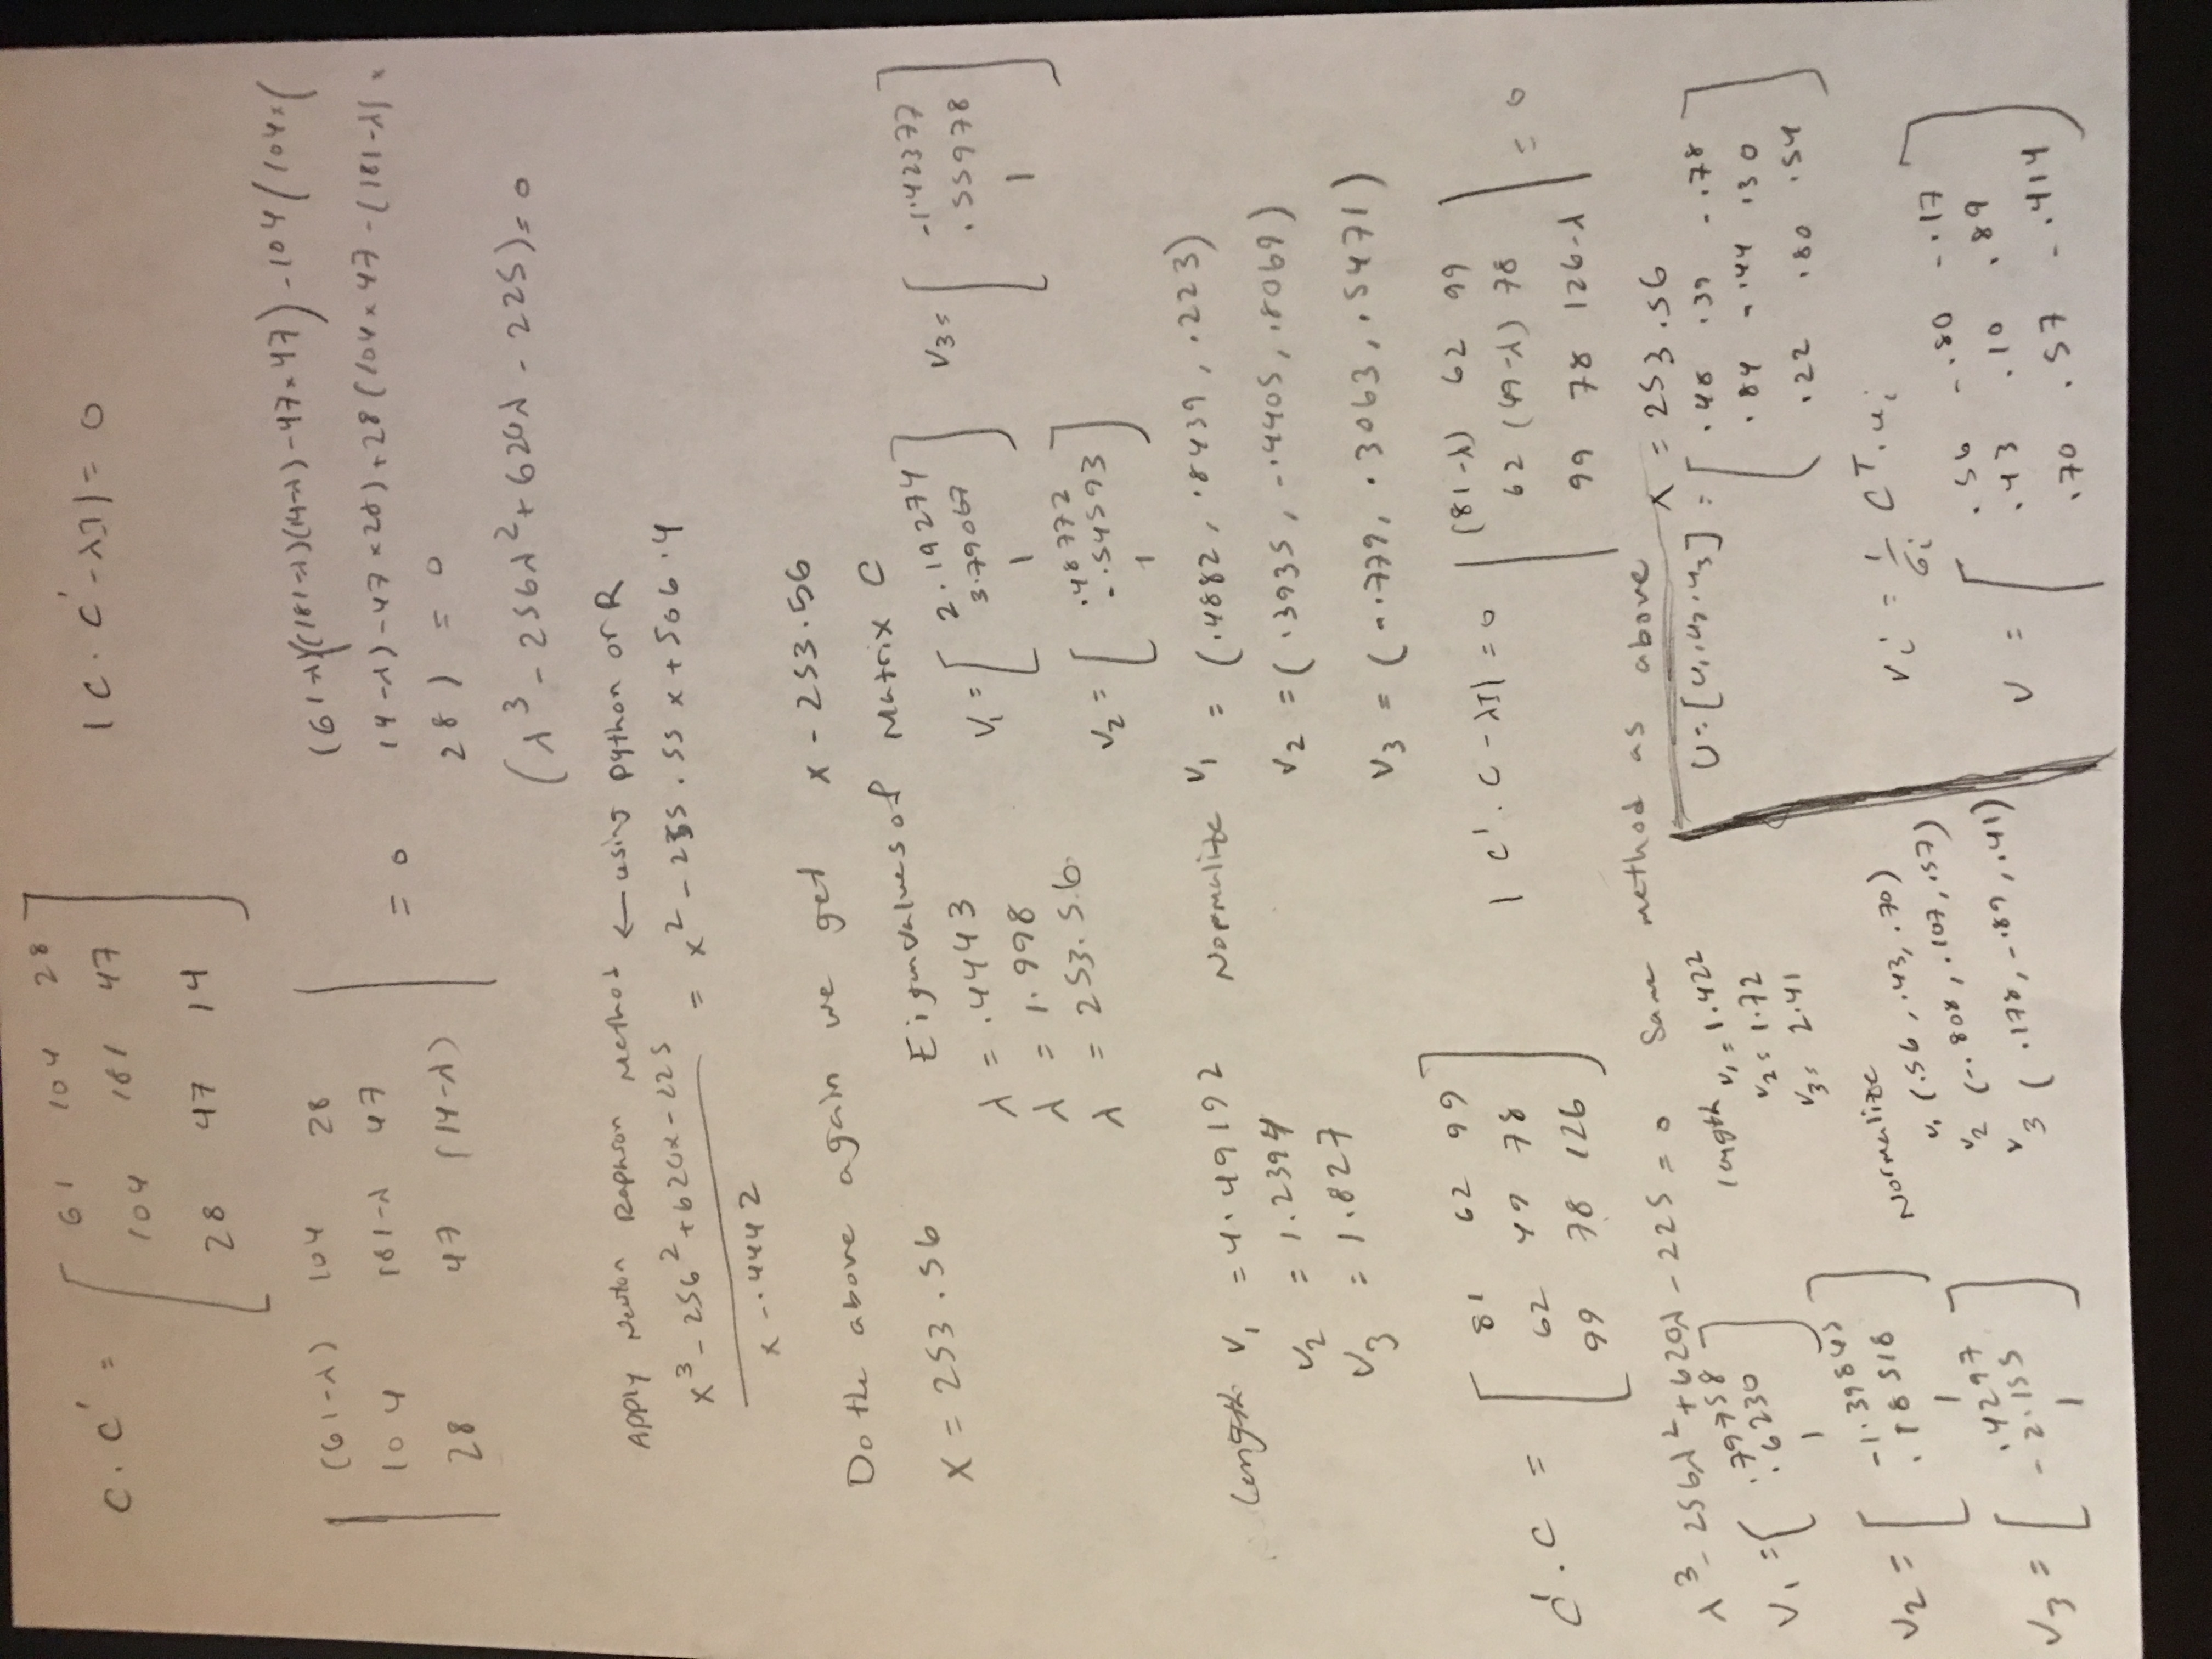
\includegraphics[scale=.1]{1}

}

\end{homeworkProblem}
\pagebreak

\begin{homeworkProblem}[Graduate Only, Extra Credit for Undergraduate Students]
 {\sf\textbf{[10 pts]} } Prove that the determinant of a matrix $A$ is the area scaling factor of the geometric transformation represented by $A$.

%%%%% Your Answer here:
\problemAnswerEnhanced{

	This was a long problem and tedious to do on latex, and I have no idea how to do the pictures on latex.
	
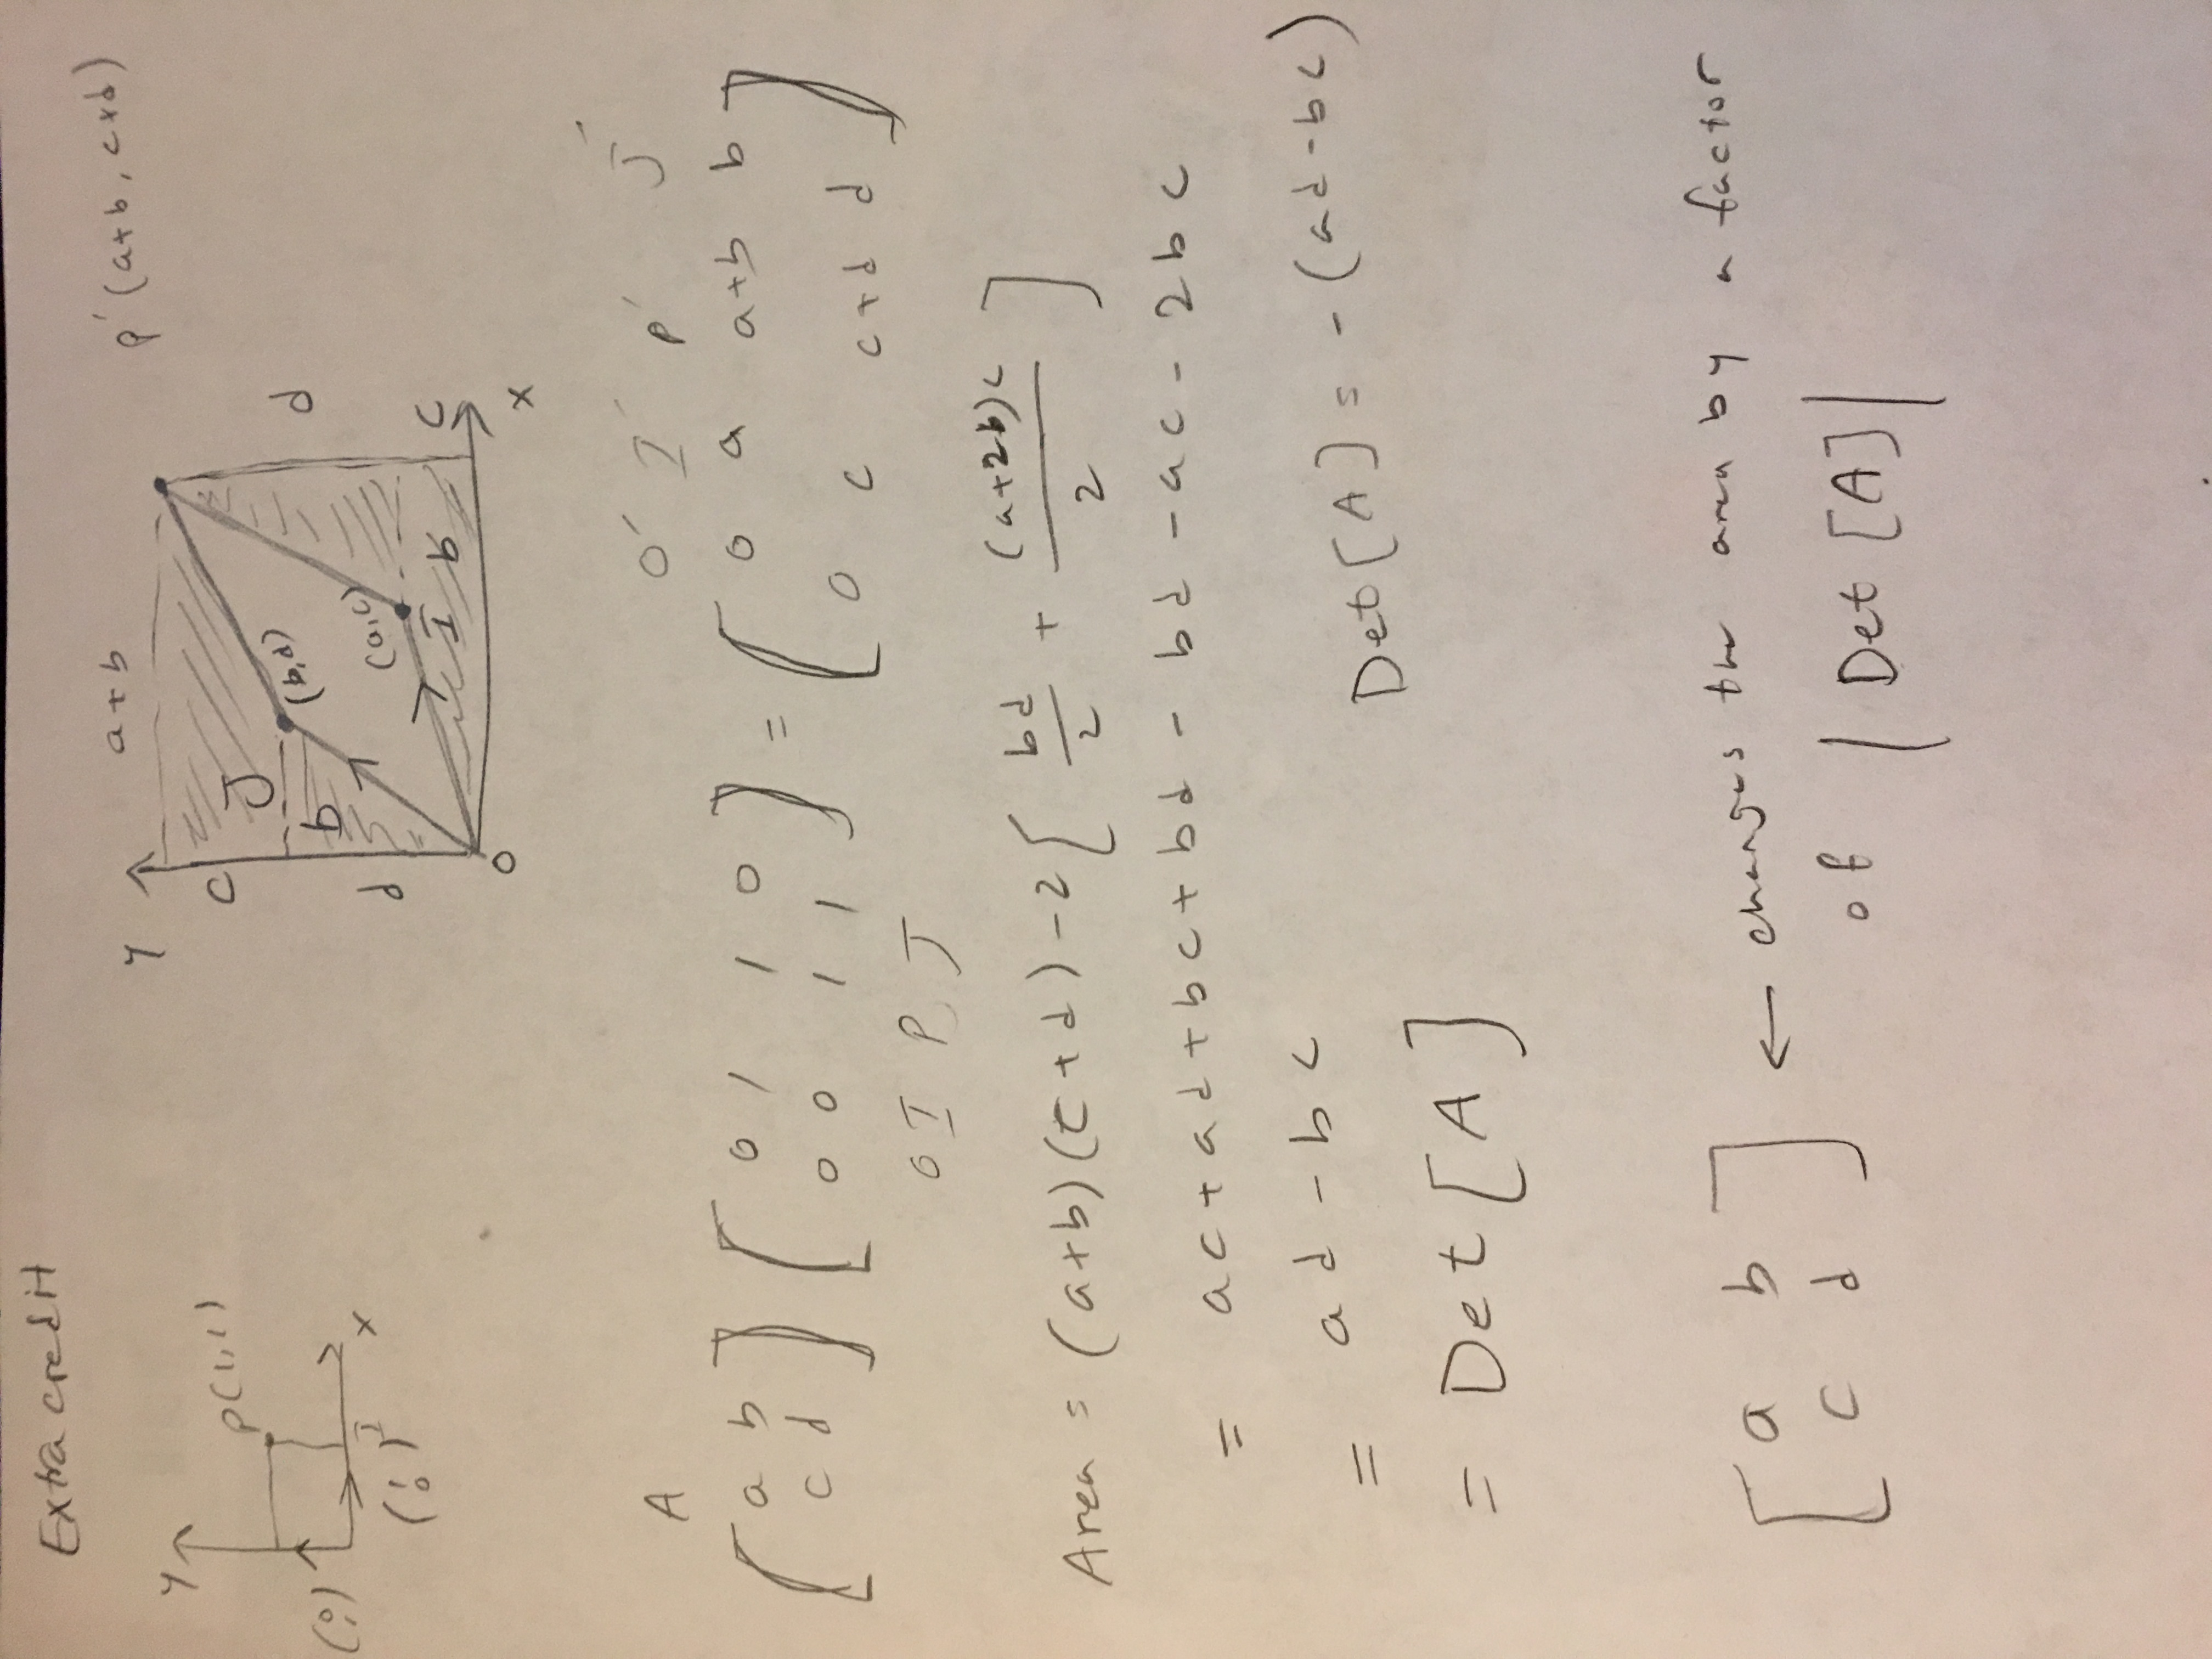
\includegraphics[scale=.1]{2}
}

\end{homeworkProblem}
\pagebreak


\end{spacing}
\end{document}

